\documentclass[preprint,authoryear,12pt]{elsarticle}

\usepackage{graphicx}
\usepackage{url}		% Display web addresses nicely
\usepackage{amsfonts,amssymb,amsbsy,amsmath,amscd}

\RequirePackage{latexsym,ifthen,theorem,booktabs}
\RequirePackage{amsfonts,amssymb,amsbsy,amsmath,amscd}
\usepackage{verbatim}
\biboptions{sort}

% Shortcuts / styling
\newcommand{\secref}[1]{Section~\ref{#1}}
\newcommand{\code}[1]{\texttt{#1}}
\newcommand{\Matlab}{{\sc Matlab}\textsuperscript{\textregistered}}
% A value with units
\newcommand{\vu}[2]{\ensuremath{#1\,\mathrm{#2}}}

\newcommand{\ud}{\mathrm{d}}
\newcommand{\dt}{\ud t}
\newcommand{\dd}[2]{{\ud #1}/{\ud #2}}

% Authors' notes
\usepackage{color}
%\newcommand{\authornote}[2]{{\bf\color{red} [#1: #2]}}
\newcommand{\authornote}[2]{{\bf [#1: #2]}}
\newcommand{\jc}[1]{\authornote{Jon}{#1}}
\newcommand{\gary}[1]{\authornote{Gary}{#1}}
\newcommand{\steve}[1]{\authornote{Steve}{#1}}

%\newcommand{\changed}[1]{\textcolor{cyan}{#1}}
\newcommand{\changed}[1]{#1}

\graphicspath{{images/}}

% Title page info
\journal{Progress in Biophysics and Molecular Biology}
\begin{document}
\begin{frontmatter}
\title{High throughput functional curation of cellular electrophysiology models}
\author[oucl]{Jonathan Cooper\corref{cor}}
\ead{jonathan.cooper@comlab.ox.ac.uk}
\cortext[cor]{Corresponding author.  Oxford University Computing Laboratory, Wolfson Building, Parks Road, Oxford, UK, OX1 3QD.}

\author[dpag]{Gary R. Mirams\fnref{jfa}}
\ead{gary.mirams@dpag.ox.ac.uk}
\fntext[jfa]{Joint first author}

\author[kcl]{Steven A. Niederer}
\ead{steven.niederer@kcl.ac.uk}

\address[oucl]{Oxford University Computing Laboratory, University of Oxford, Oxford, UK}
\address[dpag]{Department of Physiology, Anatomy \& Genetics, University of Oxford, Oxford, UK}
\address[kcl]{Biomedical Engineering Department, Imaging Sciences \& Biomedical Engineering Division, King's College London, UK}

%%%%%%%%%%%%%%%%%%%%%%%%%%%%%%%%%%%%%%%%%%%%%%%%%%%%%%%%%%%%%%%%%%%%%%
\begin{abstract}
% Avoid references & abbreviations if possible; expand if included.

% Key idea: automating the evaluation of experimental protocols for cell models enables the identification of a model that exhibits an experimentally observed phenomenon.

Effective reuse of a quantitative mathematical model requires not just access to curated versions of the model equations, but also an understanding of the functional capabilities of the model, and the advisable scope of its application.
To enable this ``functional curation'' we have developed a simulation environment that provides high throughput evaluation of a mathematical model's functional response to an arbitrary user-defined protocol, and optionally compares the results against experimental data.
In this study we demonstrate the efficacy of this simulation environment on 31 cardiac electrophysiology cell models using two test-cases.
The S1-S2 response is evaluated to characterise the models' restitution curves,
and their L-type calcium channel current-voltage curves are evaluated.
The significant variation in the response of these models, even when the models represent the same species and temperature, demonstrates the importance of knowing the functional characteristics of a model prior to its reuse.

We also discuss the wider implications for this approach, in improving the selection of models for reuse, enabling the identification of models that exhibit particular experimentally observed phenomena, and making the incremental development of models more robust.
\end{abstract}

\begin{keyword}
% Immediately after the abstract, provide a maximum of 6 keywords, using British spelling and avoiding general and plural terms and multiple concepts (avoid, for example, "and", "of").
% Be sparing with abbreviations: only abbreviations firmly established in the field may be eligible.
% These keywords will be used for indexing purposes.
cardiac electrophysiology \sep CellML \sep protocol \sep simulation
\end{keyword}

% Define abbreviations that are not standard in this field in a footnote to be placed on the first page of the article.
% Such abbreviations that are unavoidable in the abstract must be defined at their first mention there, as well as in the footnote.
% Ensure consistency of abbreviations throughout the article.
%%%%%%%%%%%%%%%%%%%%%%%%%%%%%%%%%%%%%%%%%%%%%%%%%%%%%%%%%%%%%%%%%%%%%%

\end{frontmatter}


%%%%%%%%%%%%%%%%%%%%%%%%%%%%%%%%%%%%%%%%%%%%%%%%%%%%%%%%%%%%%%%%%%%%%%
\section{Introduction}
\label{sec:intro}
%%%%%%%%%%%%%%%%%%%%%%%%%%%%%%%%%%%%%%%%%%%%%%%%%%%%%%%%%%%%%%%%%%%%%%

%%%%%%%%%%%%%%%%%%%%%%%%%%%%%%%%%%%%%%%%%%%%%%%%%%
\subsection{Aims}
\label{sec:intro-aims}
%%%%%%%%%%%%%%%%%%%%%%%%%%%%%%%%%%%%%%%%%%%%%%%%%%

Central to the philosophy of the international IUPS Physiome and Virtual Physiological Human (VPH) modelling efforts \citep{Bassingthwaighte.00:Strategies,Cooper*.10:Virtual} is the integration and coupling of existing biophysical mathematical models, that represent both specific physiological function, and how this function changes in the presence of pathologies or pharmacological agents.
This philosophy enables the development of new integrated models that represent interactions and regulatory mechanisms that span across multiple spatial and temporal scales and are intrinsic to biological systems.
These integrated models enable the study of complex feedback loops and emergent phenomena, and provide an essential tool for combining extensive disparate experimental and clinical data sets.
However, to reuse a mathematical model effectively requires both a correct representation of the original equations, and an understanding of the functional capabilities of the model.


The first of these requirements has been met through the development of community standards for representing mathematical models (e.g.\ CellML \citep{Lloyd*.04:CellML} and SBML \citep{SBML.04:Evolving}) and the publication of models in these formats in public access databases \citep{Lloyd*.08:CellML,BioModels.2010}.
These reference descriptions are tested and documented as part of the curation process to verify that they conform to language specifications, and that they can reproduce figures and results from the original publication.
To minimize the chance that error is introduced in the reproduction of paper results, the simulation protocols necessary to reproduce paper figures can also be encoded \citep[e.g.][]{Nickerson&Buist.09:physiome}. % Cut Nickerson*.08:Reference for space
This transparent process of publishing curated model equations and protocols in standard formats provides users with increased confidence that the model is a valid representation of the original work.


The availability of these models and the corresponding confidence in their implementation greatly reduces barriers for the reuse, adaptation or combination of existing models to study a specific question of interest.
By reusing existing model parameter sets and formulations it is hoped that the functionality present in the original model will be inherited in the model used for a new study.
This poses two challenges.
Firstly, with increasing numbers of models and concurrent increases in complexity, identifying the subset of models (or none at all), that exhibit a desired phenomena required for a particular study becomes increasingly challenging.
Secondly, if a new model is created it is important to confirm by simulation, rather than assume, that it maintains all of the functionality present in the reused models.
Therefore, contrary to the goals of the language standards, the increased availability of mathematical model equations, and the ease of their reuse without a good understanding of their capabilities, is likely to increase model misuse and introduce unintended errors into simulation results \citep{Smith*.07:Computational}.


Examples of many of the challenges facing model reuse within the VPH and Physiome projects are demonstrated by cardiac cell models, a field that is mature enough to have multiple generations of models and corresponding model reuse.
Cardiac electrophysiology cell models have developed over the past 50 years, routinely build on existing models and exhibit complex multiscale functionality.
Furthermore previous test cases, where only two models were compared, have demonstrated discrepancies in function between models that purport to represent a common species, cell type and temperature \citep{Niederer*.09:meta,cherry2007tale}.
The large number of cardiac cellular electrophysiology models available, representing both specific animal species but also specific regions or sub-regions of the heart, have been developed to study a diverse range of cardiac physiology, including variations in temperature, pacing rate, ionic concentrations, sex, and age \citep{Clayton*.10:Models}.
This diversity means that when approaching a new area of interest an applicable
model may already exist, however, evaluating the suitability of current models
for a specific situation is not currently readily assessed.


In this paper we consider, design and implement the infrastructure necessary to perform high-throughput \emph{functional curation} of models---subjecting a large number of existing models to commonly-used electrophysiology protocols.
Thus we may examine which of the models are capable of replicating experimentally observed results, and evaluate their suitability for reuse in future modelling studies.



%%%%%%%%%%%%%%%%%%%%%%%%%%%%%%%%%%%%%%%%%%%%%%%%%%
\subsection{Existing Tools and Extensions}
\label{sec:intro-existing-work}
%%%%%%%%%%%%%%%%%%%%%%%%%%%%%%%%%%%%%%%%%%%%%%%%%%

\begin{figure}
\begin{center} % trim l b r t
\includegraphics[trim = 4mm 28mm 8mm 0mm, clip, width=\linewidth]{schematic_v4}
\caption{Components of a functional curation system.
The steps involved are:
(1) annotate models with ontological tags;
(2) combine model with protocol mathematics and simplify;
(3) run simulation;
(4) post-process model outputs; and
(5) graphically plot results.
All interaction between the protocol definition, model equations, and simulation implementation is filtered through an interface definition, ensuring that biophysical entities and physical units are appropriately mapped.}
\label{fig:schematic}
\end{center}
\end{figure}

Functional curation requires the capacity to perform simulation protocols on multiple cell models, post-process model outputs and report the results.
The proposed implementation for functional curation is outlined in Figure~\ref{fig:schematic}.
There are three distinct types of components that need to be defined or developed.
Firstly, language components are required to provide a formal definition of model equations, simulation protocols, post-processing steps, and desired outputs.
Secondly, interface components need to be defined to allow these different languages to be translated into common variable names and units. 
Thirdly, compute components are required to interpret the languages, implement simulation protocols, perform simulations, post-process model outputs, and produce graphical plots.


Presently there are \changed{recognized community standard} languages which meet the requirements for some of the language components.
As noted above, CellML and SBML provide convenient language standards to formally define cell model equations.
Two mark-up language projects \changed{currently provide} standards for defining both model simulation protocols and graphical outputs\changed{---SED-ML \citep{SED-ML.08}, and the CellML Simulation and Graphing Metadata draft standards\footnote{\url{http://www.cellml.org/specifications/metadata/simulations} and \url{http://www.cellml.org/specifications/metadata/graphs}} \citep[CSM and CGM respectively; used in][for example]{Nickerson&Buist.09:physiome}.
These could potentially} be used for defining simulation protocols for multiple models.
\changed{However, in their current forms both languages do not have sufficient functionality for our needs.
Protocols defined in SED-ML are tightly tied to a particular model, with all references to variables being model specific, hence typically precluding the definition of a single protocol that can be applied to multiple models; it is thus incapable of supporting the necessary interfacing.
Current implementations of both languages only support `time course' simulations---a single solve of model equations.
Neither language is capable of expressing parameter sweeps, or any general form of repeated simulation (although such features are planned for later versions of SED-ML).
Finally, neither language supports anything more than extremely basic post-processing steps.}\footnote{The only post-processing supported is essentially `map'-type operations, applying an operator element-wise to one or more arrays of outputs to produce a new array. CGM also includes some limited filtering capabilities.}



The interface between the protocol language, model equations, and simulation platform is a key aspect of functional curation, in order to support running a protocol on multiple models and coherently comparing the results.
Since variable names in models are arbitrary, a mapping is required labelling variables so as to uniquely relate them to a biophysical quantity or protocol construct.
Both SBML and CellML support such labelling through RDF annotations, using terms taken from ontologies \citep{Novere&Finney.05:simple,Beard*.09:CellML}.


To compare outputs correctly requires a second interface component for interpreting and converting the physical units associated with variables, since again models vary in the units used for the same quantity.
Every quantity in a model and protocol must have its units indicated, and suitable scaling conversions can be added automatically \citep{Cooper&McKeever.07:Model-driven}.
More complex conversions may also be required, utilizing biophysical knowledge to define conversion functions that reference quantities within the model using ontological terms, as above.
A common case within cardiac modelling is converting ionic currents, for example to convert a current defined in Amperes per unit area (of a cell membrane) to a current defined in Amperes requires multiplication by the cell surface area \citep{Cooper*.11:Considerations}.


\changed{While there are several simulation environments available that support simulation of CellML models \citep[see][]{Garny*.08:CellML}, none have the capabilities required of a functional curation system.
Both COR \citep{COR} and OpenCell \citep[formerly known as PCEnv,][]{Garny*.08:CellML}, for example, support only time-course simulations of single models through a graphical user interface, and Chaste \citep{Chaste.CPC} has primarily used CellML models within cardiac tissue simulations.
We are therefore developing a new open source system, based on and extending the Chaste simulation platform, in order to provide high throughput evaluation of models' functional responses to arbitrary user defined protocols.
Since available protocol languages, and in particular SED-ML, do not provide sufficient expressivity to encode the protocols we wish to run (as described above), we are also proposing novel language features to support such uses.
We focus on complex post-processing and model modifications, which have not been central in the development of existing languages.}


%\changed{It must be emphasized that we are not seeking to define a new protocol language in competition to SED-ML.
%Rather, we are prototyping language features and demonstrating their effectiveness and ease of implementation, in order to provide detailed concrete proposals for future SED-ML development.
%While our system currently uses our own language, therefore, it is hoped that a future version will be based on SED-ML instead.}


The features of \changed{our functional curation implementation, and particularly the protocol language features incorporated within it}, are detailed in \secref{sec:methods}.
Case studies demonstrating the capabilities of the system are described in \secref{sec:case-studies}, and the results shown in \secref{sec:results}.
Finally, in \secref{sec:discussion} we discuss some salient features of our solution within the wider context of physiological modelling, finishing with some concluding thoughts in \secref{sec:conclusion}.



%%%%%%%%%%%%%%%%%%%%%%%%%%%%%%%%%%%%%%%%%%%%%%%%%%%%%%%%%%%%%%%%%%%%%%
\section{Methods}
\label{sec:methods}
%%%%%%%%%%%%%%%%%%%%%%%%%%%%%%%%%%%%%%%%%%%%%%%%%%%%%%%%%%%%%%%%%%%%%%

In this section we outline our proposed implementation of functional curation, treating the steps in the order given in Figure~\ref{fig:schematic}, followed by two test cases that demonstrate the utility of this method.
Our implementation is guided by twin aims: to produce a system with sufficient expressive power to be able to run a range of complex protocols, and yet also for the protocol language to be relatively straightforward to implement.
% This is because we are not intending that everyone should use our system (in which case recommending the use of a general-purpose environment such as \Matlab{} would be sufficient).
% Rather, just as has been done with CellML and SBML, we wish to develop a standard that others will use.
% This is required for take-up within the community, and for protocol descriptions to become commonplace alongside publications.
% Another principle arising from this is that it should be as easy as possible for model authors to write protocol descriptions in our language.
% We will therefore distinguish features of the protocol language itself from our prototype implementation.
% Our implementation efforts are proceeding in an iterative agile fashion \citep{Chaste.08}, building up functionality as required.
%We have started with the `back-end' reference implementation, in order to be able to run some initial protocols and demonstrate the utility of the approach.
%At the time of writing, this implementation based on Chaste \citep{Chaste.CPC} has been created and core functionality completed.
%The language syntax however has not been finalized, and so our description will focus on the key language concepts, rather than details of how they are expressed.
The software is open source, and available to download from \url{http://www.comlab.ox.ac.uk/chaste}.

% Firstly we discuss the interface components for coupling protocol, model, and simulation environment, along with annotation of models from the repository to support this.
% We then describe how the mathematics from the model and protocol are combined to produce the equations that are to be solved, and then how solving these equations is structured in a complex simulation, which is run to produce output arrays.
% Next we describe the post-processing functionality available to generate derived outputs from these, and finally how graphical plots of these outputs may be specified for visual evaluation.
% 
% The protocol language is presented as a single entity, although as can be seen from Figure~\ref{fig:schematic} it has several components, some of which could be independent, and potentially sourced from elsewhere.
% This is particularly the case for the definition of graphical outputs.
% All other components, however, make use of the core mathematical functionality, and there is some overlap, for example with shared variables.
% Furthermore, post-processing functions could be interleaved with the simulation definition, as we discuss in \secref{sec:discussion}.
% We will nevertheless make use of other standards where appropriate, e.g.\ leveraging MathML\footnote{\url{http://www.w3.org/TR/MathML2/}} to denote basic mathematics.
% 
% Finally, we define two test case protocols that are applied to a repository of cardiac cell models to provide an application context for our proposed functional curation method.

%%%%%%%%%%%%%%%%%%%%%%%%%%%%%%%%%%%%%%%%%%%%%%%%%%
\subsection{Language Interfaces}
\label{sec:methods-interfaces}
%%%%%%%%%%%%%%%%%%%%%%%%%%%%%%%%%%%%%%%%%%%%%%%%%%


Applying a protocol language to a repository of arbitrary models requires a machine readable mapping of variable names and units between the protocol description and each of the models.
This is achieved through metadata labelling of variables within the cell model files and the development of functional unit conversion.

%%%%%%%%%%%%%%%%%%%%%%%%%%%%%%%%%%%%%%%%%%%%%
\subsubsection{Metadata Labelling}
\label{sec:methods-ontologies}
%%%%%%%%%%%%%%%%%%%%%%%%%%%%%%%%%%%%%%%%%%%%%

To apply the protocols defined in the protocol language onto existing models requires a translation of variable references in the protocol to the variable names in the model, allowing the protocol to interface with a model purely at the mathematical level.
Rather than identifying variables by name, or by location within the model file, we thus require models to be annotated with biological metadata, using an ontology to provide standard names for entities of interest.
This technique is independent of a specific ontology---providing that the model and protocol use the same ontology terms.
%It also offers the potential for more straightforward support of multiple modelling languages, since the protocol language itself does not need to `know' how a modelling language is structured, providing it supports such annotations (as both SBML \citep{Novere&Finney.05:simple} and CellML \citep{Beard*.09:CellML} do).

%The first stage of running a protocol is therefore to prepare the models to be used by annotating them with terms from the chosen ontology.

%%%%%%%%%%%%%%%%%%%%%%%%%%%%%%%%%%%%%%%%%%%%%
\subsubsection{Unit Conversion}
\label{sec:methods-units}
%%%%%%%%%%%%%%%%%%%%%%%%%%%%%%%%%%%%%%%%%%%%%

The diversity of modelling strategies and frameworks, compounded with the range of measurement techniques means that the same biological function can be represented by equations with incompatible units.
This can be demonstrated with a cell membrane current as described above, or more subtly a concentration flux from the cytosol to an organelle with the units of Mole per litre per second does not explicitly state the volume of the concentration.
This means it could be a concentration from the cytosol or the organelle.
If comparing two fluxes from two models with these units, they must be with reference to the same volume for valid comparisons to be made.
We use the framework described in \citep{Cooper*.11:Considerations} to support the definition of units conversion functions, which may use the values of model variables (identified by ontological labels) to perform complex conversions and hence enable meaningful comparisons between models.

%%%%%%%%%%%%%%%%%%%%%%%%%%%%%%%%%%%%%%%%%%%%%%%%%%
\subsection{Determining Equations for Simulation} 
\label{sec:proto-step2}
%%%%%%%%%%%%%%%%%%%%%%%%%%%%%%%%%%%%%%%%%%%%%%%%%%

The equations to be simulated will not always be identical to those in the original reference model implementation.
Firstly, the model equations must be changed to impose boundary and initial conditions.
Setting initial conditions may take the form of setting the values of model variables at the start of a simulation, or additional equations may be added to calculate suitable initial conditions from other parameters, including the results of previous simulations.
Thus the protocol language includes the ability to represent mathematical equations, and the same kinds of equations as might appear in a model.
Setting `boundary conditions' requires this ability to a greater extent, and may also involve replacing parts of the model with new equations.
For example, the trans-membrane potential $V$ in an electrophysiology model is generally a time-varying state variable defined by an ordinary differential equation (ODE).
If a `voltage clamp' protocol is applied, however, the value of $V$ is instead fixed by the protocol, and its defining ODE should be removed from the model to avoid a conflict.


Secondly, the protocol language allows the specification of `outputs'---those variables whose values over the course of the simulation should be recorded for post-processing.
Often it will be desirable to save only the relevant subset of the data produced by a model, and so the variables to be recorded, and their sampling intervals, should be specified.
These outputs may not appear directly in the model, in which case new equations need to be added, as above.
Also, it may not be necessary to simulate all of the model equations in order to determine the desired outputs.
For some protocols, this may even mean that there is no time-varying component to the simulation at all, for example when evaluating the substrate sensitivity of rapid steady state transporter models or enzyme kinetics.
Faster simulations may therefore be achieved in these cases by analysing the model equations and removing those which are not required in computing the outputs.


Standards are currently available within existing languages for defining the numerical algorithm and algorithm parameters for evaluating a model.
Both SED-ML and CSM allow time-course simulations to be specified with various numerical methods and parameters thereof, and we have adopted such standards within our language.


Solving repeated time-course simulations while adjusting input information allows
simulations to sweep parameters for fitting, or to characterise a response as a
function of an input.
In order to allow these more complex simulations, we use the
ideas of the nested simulation proposal for SED-ML \citep{Bergmann.10:Simple}.
This allows loops to be applied to simulations, and with each iteration of the
loop a parameter of the model or protocol is altered.
This mechanism enables the
implementation of a parameter sweep, while multiple layers of nesting then
allows for multi-dimensional sweeps.



%%%%%%%%%%%%%%%%%%%%%%%%%%%%%%%%%%%%%%%%%%%%%%%%%%
\subsection{Post-processing}
\label{sec:proto-pp}
%%%%%%%%%%%%%%%%%%%%%%%%%%%%%%%%%%%%%%%%%%%%%%%%%%
% Post-processing

Post-processing of simulation outputs (and of post-processed outputs) must be included in a protocol language used for functional curation.
Often complex processing must be performed in order to obtain the quantities of interest.
Careful balancing of this goal of expressivity, with the need to minimise the burden for implementations, is therefore required.
We thus define a small set of elementary language features, which can be combined within the language itself to achieve complex behaviour.
Any implementations of the language then need merely to support the basic set.


The form of the model output data strongly influences the types of the elementary language features.
Previous languages, including SED-ML and CellML-based languages, only supported single simulations, with simulation results therefore stored as single dimension arrays.
Our protocol language supports nested simulations, which leads naturally to outputs being represented as n-dimensional arrays of double-precision floating point values.
The number of dimensions is given by the number of levels of nesting, and the size of each dimension by the number of (sampling) points in the range over which the corresponding simulation loops.


We therefore define an array-based language building on this single data-type.
Many similar, and general purpose, array-based languages exist \citep[e.g.][]{Scholz.03:Single,Jenkins.93:Nial,McGraw*.85:SISAL,Burke.96:J}, perhaps most notably \Matlab, NumPy \citep{Oliphant.07:Python}, and APL \citep{Iverson.62:APL}.
To reduce the implementation burden and complexity our language will be less powerful, with features only added if necessary to express desired protocols.
A key feature is that arrays cannot be modified once created (i.e.\ it is a pure functional language), which simplifies processing.
Each operation in the language takes arrays as input, and produces new arrays as output.
The language supports the definition of functions, and collections of functions, in order to allow libraries of common operations to be developed, thus reducing the burden for protocol authors.


The language includes basic arithmetic operations that are available within MathML, and used by both SBML and CellML.
Supporting these should therefore not impose any additional burden on implementations.
In addition to this, the language contains operations for working with n-dimensional arrays.
There are just six foundational operations, from which all of the post-processing required by our case studies can be constructed.
\begin{description}
\item[Array creation]
  Arrays can be created directly within the protocol language.
  As array content can not be changed, arrays must be populated at initiation.
  This can be done simply by listing the entries, or defining the values as functions of the element indices, existing arrays, or as constants.
\item[Map]
  This operation allows basic arithmetic functions, (i.e.\ \code{+}, \code{-}, \code{>}, \code{<}, \code{abs}, etc.) to be applied element-wise to one or more arrays.
\item[Fold]
  This allows an operation to be performed on each element along one dimension of an array to produce a single value, yielding a result array with one fewer dimensions than the input.
  For example addition along an array will produce the sum, or a comparison along the array can be used to determine the maximum or minimum value.
\item[Find]
  This locates non-zero entries within the input array, and returns an array of their indices.
  The result array can be used as an input to the \code{index} operation.
\item[Index]
  This generates a new array consisting only of those entries in the input whose indices appear in the indices array supplied.
\item[Views]
  New arrays may be created by taking sub-arrays of existing arrays.
  These can contain contiguous elements, or be formed by striding across the input, taking every second element along one dimension for example.
\end{description}


A key feature, reflected also in the core language operations, is that functions in our language can be agnostic as to the dimensionality of the inputs.
This allows them to function without the number of dimensions being hard-coded, and hence permits multi-dimensional parameter sweeps without any limit on the number of parameters being varied.


%%%%%%%%%%%%%%%%%%%%%%%%%%%%%%%%%%%%%%%%%%%%%%%%%%
\subsection{Graphical Outputs}
\label{sec:proto-results}
%%%%%%%%%%%%%%%%%%%%%%%%%%%%%%%%%%%%%%%%%%%%%%%%%%

Finally, to formalise the link between model equations and results as they might appear in a published paper, it must be possible to define the graphical figure outputs produced from the model outputs and subsequent post-processing steps.
In this area we will also leverage existing work, since both SED-ML and CGM contain features for describing graphs (our prototype implementation currently uses hard-coded gnuplot scripts).
Results can also be output to file if further processing for comparison is required.
Again little has thus far been done in this area, but formats such as BiosignalML\footnote{\url{http://www.embs.org/techcomm/tc-cbap/biosignal.html}} or SBRML \citep{Dada*.10:SBRML} would be potential targets for future work.



%%%%%%%%%%%%%%%%%%%%%%%%%%%%%%%%%%%%%%%%%%%%%%%%%%
\subsection{Case Studies}
\label{sec:case-studies}
%%%%%%%%%%%%%%%%%%%%%%%%%%%%%%%%%%%%%%%%%%%%%%%%%%

To demonstrate the utility of functional curation and show the functionality
enabled through the proposed combination of languages, interfaces, and computation
code we have performed two standard protocols, specifically the S1-S2 and the
I$_\textrm{CaL}$ current--voltage plot, on a repository of cardiac cell models.


%%%%%%%%%%%%%%%%%%%%%%%%%%%%%%%%%%%%%%%%%%%%%
\subsubsection{S1-S2 Protocol}
\label{sec:intro-s1s2}
%%%%%%%%%%%%%%%%%%%%%%%%%%%%%%%%%%%%%%%%%%%%%

The first test case is the ``S1-S2'' restitution curve protocol first described by
\citet{nolasco1968graphic}. This protocol consists of a series of stimuli applied
at a steady pacing cycle length (S1) until action potentials become regular
(reach a limit-cycle, mathematically speaking), followed by a single stimulus
applied at a different cycle length (S2).
The action potential duration resulting from the S2 stimulus is plotted against
the diastolic interval (DI) preceding that stimulus, as shown in
Figure~\ref{fig:S1S2Intro}.

\begin{figure}
\begin{center}
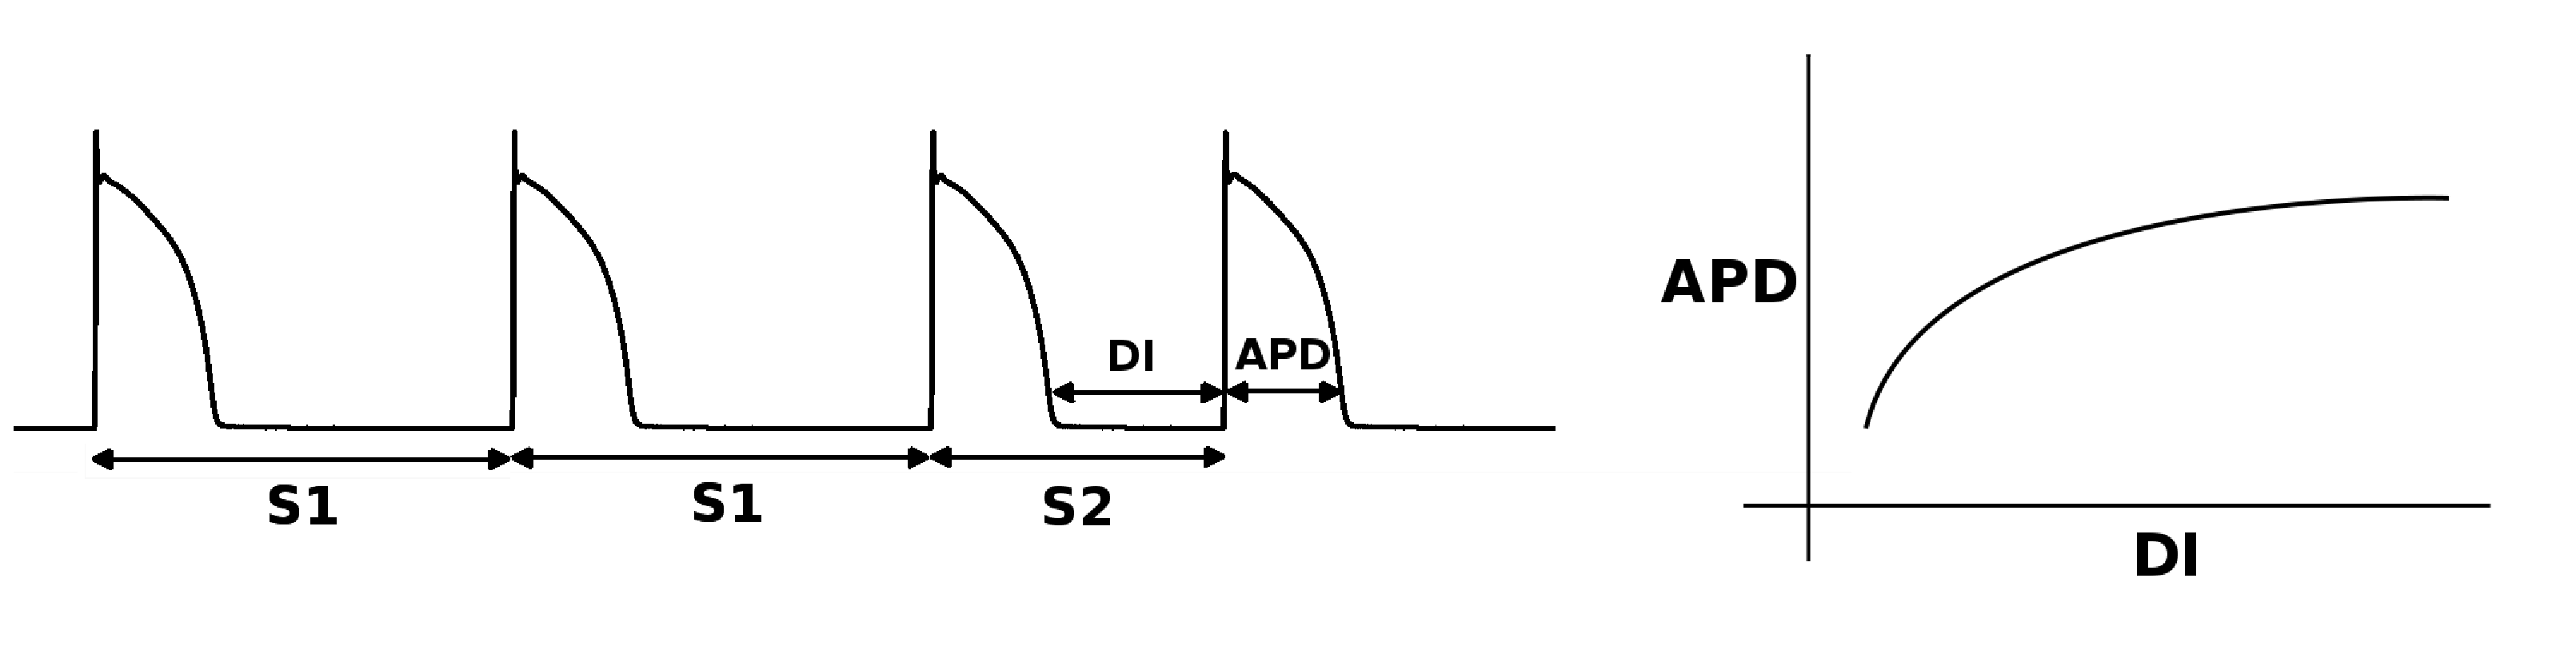
\includegraphics[width=1.0\linewidth]{S1S2}
\caption{Left: the S1-S2 pacing protocol with S1, S2 pacing cycle lengths,
diastolic interval (DI) and action potential duration (APD) marked. Right: the
axes and shape of a typical restitution curve, formed by repeating the protocol
with varying S2 intervals, for a fixed choice of S1.}
\label{fig:S1S2Intro}
\end{center}
\end{figure}

Experimental restitution slopes for healthy cells typically follow the trend
shown in Figure~\ref{fig:S1S2Intro}, with APD shortening following a smaller DI,
and tending to a steady size as the DI is increased.
%It is suggested that a steeper restitution curve is associated with increased
%risk of arrhythmia \citep{kim2002action}, and vice-versa
%\citep{garfinkel2000preventing}.


This protocol was implemented as follows.
Firstly, to allow the protocol language to interact with the models the CellML implementations of these models were annotated with metadata to identify the variables used in the protocol definition.
These included the transmembrane potential, simulation time, and the stimulus current, amplitude, duration, and period variables. 


The simulation definition for this protocol consists of two nested loops.
The outer loop modifies a variable specifying the S2 interval, and the inner loop performs a time-course simulation.
For each inner loop iteration the protocol defines all of the state variables to be initialised to be on the limit cycle for S1 pacing.
For each outer loop the period of the stimulation current is incremented to adjust the S2 interval.
As the S1-S2 protocol is based solely on the membrane potential transient only the membrane potential is specified as being output every \vu{1}{ms} within the problem definition.
The membrane potential output is thus a 2 dimensional array in time and S2 interval.


The final outcome of the S1-S2 protocol is a plot of APD against DI.
These quantities are evaluated by a single \code{apd} function, given voltage $V$ and time $t$ as inputs.
It has been designed to be dimension-agnostic, supporting input voltage traces from arbitrarily nested simulations.
The function operates on a $N$ dimensional $V$ array and a $1$D time array to produce a $N$ dimensional APD array, where the time dimension from the $V$ array has been replaced with a dimension corresponding to the maximum number of APs detected in one time-course simulation.\footnote{%
For the purposes of this study, entries corresponding to simulations with fewer APs are padded with an arbitrary value.}


We note a few salient features of how the computation is performed here; full details can be found in the online supplement.
Firstly, the start of each AP is identified by finding local maxima of the gradient of $V$.
Since array operations process the whole array, in order to determine features of individual APs (rather than of a whole time-course) many steps work on extended arrays with an extra dimension varying over AP number (i.e.\ its extent is the maximum number of APs recorded in one simulation).
Having identified the peak and resting potential for each AP (using local maxima and minima functions), linear interpolation, again a function defined in terms of the basic post-processing operations, is used to locate the first times before and after each peak where the resting potential is reached, and these times are taken as the start and end of each AP; the difference between them is the APD.
Finally, the DIs are calculated by taking the element-wise difference between two arrays: the first containing the intervals between AP starts, and the second being a sub-array of the APDs, with the last removed for each run.


We also use the post-processing functionality to perform some filtering of these post-processed results.
Firstly, we extract the first DI and the second APD for each S2 interval, since these reflect the AP produced by the S2 stimulus.
\changed{Secondly we remove entries with a very small or negative DI.
A stimulus at a negative DI could induce a full early after depolarization.
Alternatively at a small or negative DI the stimulus current itself could form a small depolarization, and cause a subsequent delay in repolarization of the last S1 AP.
Neither case is part of a standard experimental S1-S2 protocol, so we remove them from the post-processing.}


%%%%%%%%%%%%%%%%%%%%%%%%%%%%%%%%%%%%%%%%%%%%%
\subsubsection{ICaL Voltage Clamp Protocol}
\label{sec:intro-ical}
%%%%%%%%%%%%%%%%%%%%%%%%%%%%%%%%%%%%%%%%%%%%%

The second test case is based on the generation of L-type calcium channel current--voltage (IV) curves, for different extracellular calcium concentrations.
The L-type calcium channel current's reversal potential will depend on the difference between the intra- and extra-cellular calcium concentrations.
The channel also inactivates in response to an accumulation of intracellular calcium, changing the cellular action potential duration accordingly \citep{grandi2009theoretical}.
The extracellular calcium concentration dependence of the L-type calcium channel therefore has important cell-level effects.
The IV curve protocol consists of clamping the voltage to a `holding potential' (in the literature this is between \vu{-50}{mV} and \vu{-40}{mV}) followed by a step change to a `testing potential'.
We illustrate the principle of this protocol in Figure~\ref{fig:ICaLIntro}.

\begin{figure}
\begin{center}
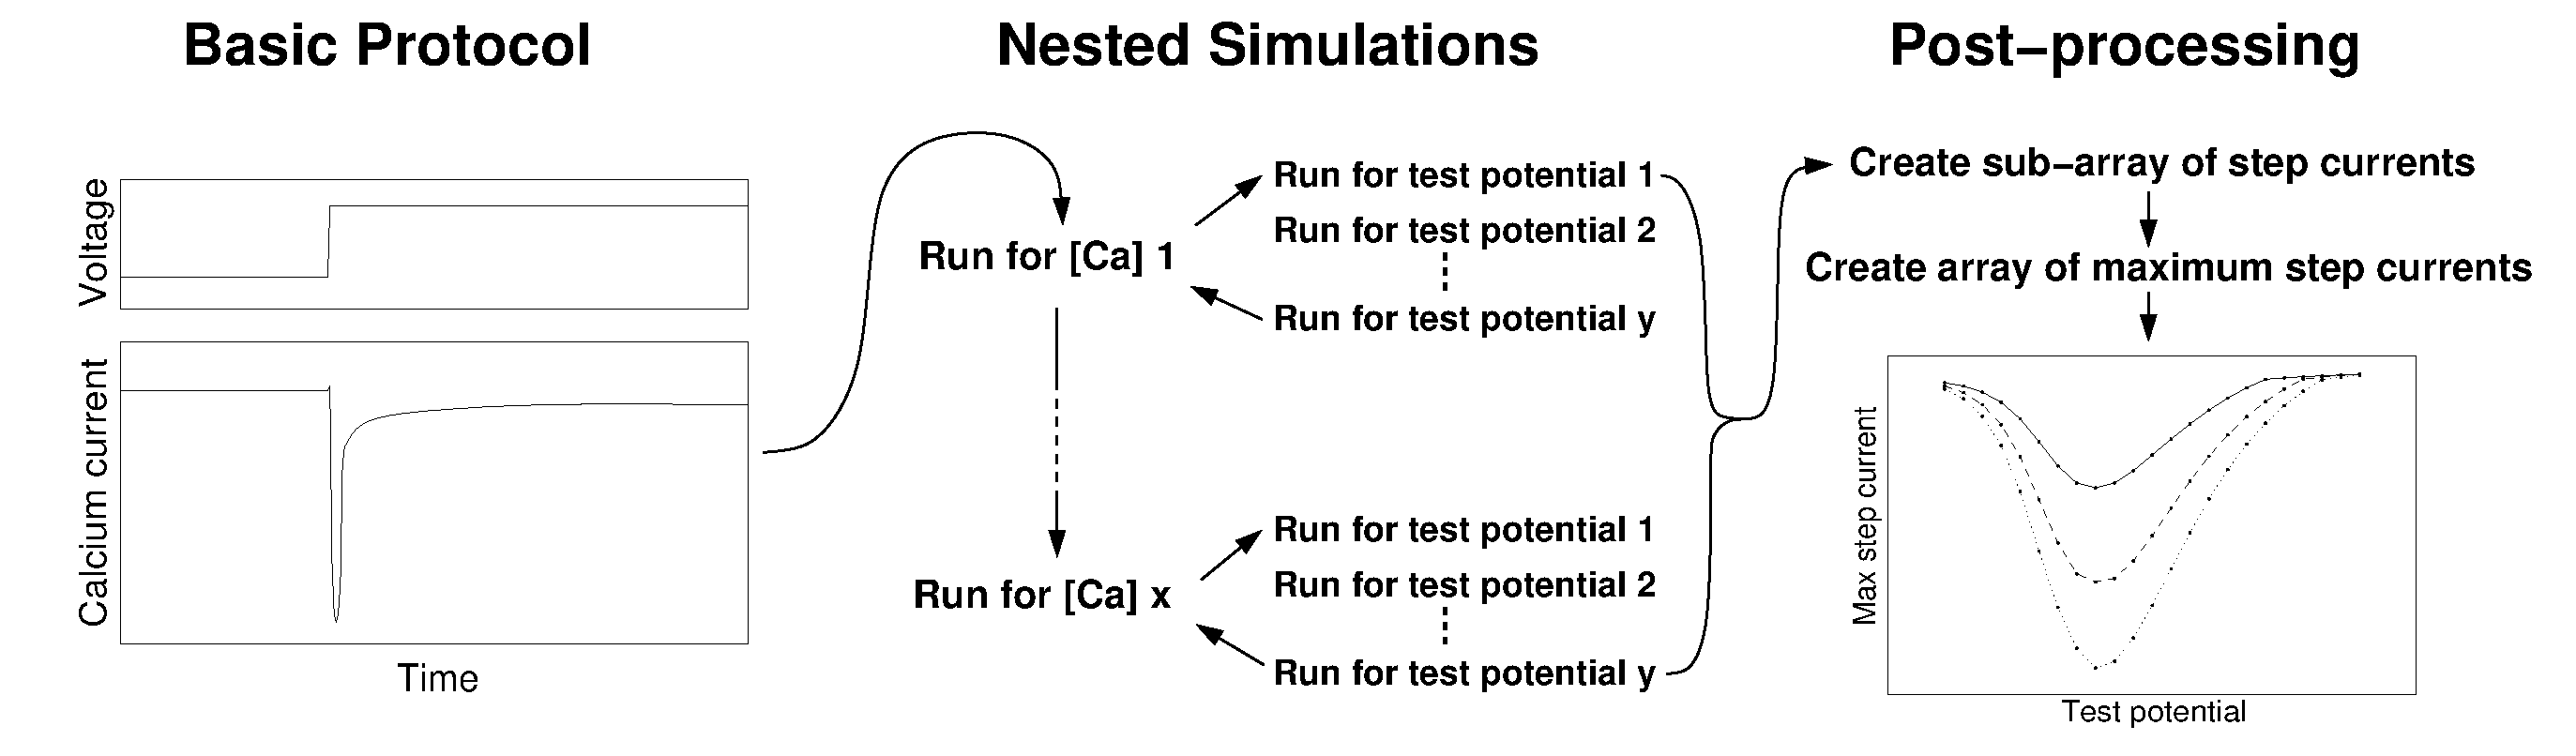
\includegraphics[width=1.0\linewidth]{ICaLIntro}
\caption{Left: a voltage clamp and the resulting L-type calcium current.
Centre: nested simulations formed by repeating the protocol for different extracellular calcium concentrations, and also different test potentials.
Right: post-processing steps and plotting.}
\label{fig:ICaLIntro}
\end{center}
\end{figure}

\changed{The largest magnitude of the L-type calcium current produced as a result of the voltage step (the minimum since the current is negative) is plotted for each test potential.}
The protocol is carried out at varied extracellular calcium concentrations (we have chosen 50\%, 100\% and 150\% of the models' default values).


Since both the test potential and extracellular calcium concentration are varied, this protocol is represented by three nested loops.
The outer loop modifies the extracellular calcium concentration, the middle loop modifies the test potential, and the inner loop performs the time-course simulation.
A time-dependent modification occurs at $t=0$ and the holding potential is changed to the test potential (which in this case depends on the state of the middle-loop, see Figure~\ref{fig:ICaLIntro}).


In the protocol definition the membrane potential is specified as a protocol input parameter, with time and the L-type calcium current set as outputs, to be recorded every \vu{0.05}{ms} in order to capture the fast transient behaviour of the current.
In this case the whole model is not required and the model and protocol are combined to produce a much reduced set of equations for simulation, as described in \secref{sec:proto-step2}.


Despite this protocol having an extra level of complexity with an additional nested loop in the simulation definition, the post-processing is much simpler.
Firstly a \code{map} on the time array produces an array containing non-zero values only where the time is greater than zero, i.e.\ after the test potential step was applied.
Applying \code{find} to this array yields the indices of these entries, which can be used to \code{index} the L-type calcium current array, giving a sub-array containing just \changed{the currents resulting from the voltage steps (``step currents'')}.
A minimum function is created by using a \code{fold}, applied to the step currents array, and the result allocated to a new array for plotting.


%%%%%%%%%%%%%%%%%%%%%%%%%%%%%%%%%%%%%%%%%%%%%
\subsubsection{Model Repository}
\label{sec:intro-models}
%%%%%%%%%%%%%%%%%%%%%%%%%%%%%%%%%%%%%%%%%%%%%

The two test cases are performed on a repository of cardiac cell models representing Purkinje, atrial and ventricular cells, shown in Table~\ref{tab:CellModels}.
These models represent a broad section of available cardiac cell models and provide a comprehensive test bed for evaluating the utility of functional curation.
The results of this evaluation appear in the next section.

\begin{table}
\begin{center}
\caption{Cardiac electrophysiology models used in this study.}
\label{tab:CellModels}
\begin{tabular}{l l l}
\toprule
Model & Species & Cell Type \\
\midrule
%\citet{aslanidi2009mechanisms} & Rabbit & Atrial\\
\citet{aslanidi2009optimal} & Dog & Purkinje \\
\citet{beeler1977reconstruction} & Mammalian & Ventricular\\
%\citet{benson2008canine}?? & Dog & Ventricular \\
%\citet{bernus2002computationally}?? & Human & Ventricular \\
\citet{bondarenko2004computer} & Mouse & Ventricular \\
%\citet{clancy2002na} & ??LR-based & Ventricular \\
\citet{corrias2011ionic} & Rabbit & Purkinje \\
\citet{courtemanche1998ionic} & Human & Atrial\\
\citet{decker2009properties}	 & Dog & Ventricular\\
\citet{earm1990model}	& Rabbit & Atrial\\
\citet{espinosa1998}	& Rat & Ventricular \\
\citet{faber2000action} &  Mammalian & Ventricular\\
\citet{fink2008contributions}	& Human & Ventricular \\
\citet{fox2002ionic}	& Dog & Ventricular\\
\citet{grandi2010novel}	& Human & Ventricular \\
\citet{hilgemann1987excitation}	& Rabbit & Atrial\\
\citet{hund2004rate}	& Dog & Ventricular\\
\citet{iribe2006modulatory} & Guinea-pig & Ventricular\\
\citet{iyer2004computational}	& Human & Ventricular \\
\citet{iyer2007mechanisms}	& Human & Ventricular \\
%\citet{jafri1998cardiac} &  Mammalian & Ventricular\\
%\citet{kneller2002time}?? & Dog & Atrial\\
%\citet{li2010mathematical} & Mouse & Ventricle\\ Falls over in S1-S2 protocol.
\citet{lindblad1996model} & Rabbit & Atrial\\
\citet{livshitz2007regulation}	& Dog & Ventricular \\
\citet{luo1991model} & Guinea-pig & Ventricular\\
\citet{mahajan2008rabbit}& Rabbit & Ventricular\\
%\citet{maleckar2008mathematical} & Human & Atrial\\ Falls over in ICaL protocol.
\citet{matsuoka2003role} & Guinea-pig & Ventricular\\
\citet{noble1991role}	& Guinea-pig & Ventricular\\
%\citet{noble1998improved}	& Guinea-pig & Ventricular \\Falls over in ICaL protocol.
%noble2001 \gary{No ref available? Remove?} & Guinea-pig & Ventricular \\
%\citet{nygren1998mathematical} & Human & Atrial\\
\citet{pandit2001mathematical} & Rat & Ventricular\\
\citet{pasek2008model} & Guinea-pig & Ventricular\\
\citet{priebe1998}	& Human & Ventricular \\
%\citet{puglisi2001labheart}?? & Rabbit & Ventricular\\
%\citet{ramirez2000mathematical}?? & Dog & Atrial\\
\citet{sakmann2000distribution}& Guinea-pig & Ventricular \\
\citet{shannon2004mathematical} & Rabbit & Ventricular\\
%\citet{shaw1997electrophysiologic} & ??LR-based & Ventricular\\
\citet{tentusscher2004}& Human & Ventricular\\
\citet{tentusscher2006}& Human & Ventricular\\
%\citet{wang2008mathematical} & Mouse & Ventricular\\
\citet{winslow1999mechanisms}	& Dog & Ventricular\\
\bottomrule
\end{tabular}
\end{center}
\end{table}






%%%%%%%%%%%%%%%%%%%%%%%%%%%%%%%%%%%%%%%%%%%%%%%%%%%%%%%%%%%%%%%%%%%%%%
\section{Results}
\label{sec:results}
%%%%%%%%%%%%%%%%%%%%%%%%%%%%%%%%%%%%%%%%%%%%%%%%%%%%%%%%%%%%%%%%%%%%%%

To demonstrate the ability of the protocol language, interfaces and
simulation environment to enable functional curation of a repository of
models we have applied the two test protocols above to 31 cell models.

% \gary{Additional labelling of the L-type calcium current allows the recording of
% this current in response to a voltage clamp.} 
% A set functional conversion equations is defined for the known units of the L-type calcium current, which could be generalised to any membrane current.  
% Using these metadata, C++ files compatible with Chaste were generated for each of the models, as described by \citet{Cooper*.11:Considerations}.
% In this process unit conversion is performed automatically with all input parameters defined in ms, mV and mM converted into the cell models native units and all outputs converted into ms, mV and $\mu$A$/cm^2$.
% The metadata labelling of the models described here can readily be extended and has recently being used to automate the application of drug-induced ion channel blockade \citep{mirams2011}.

In both case studies the differential equations are solved using CVODE \citep{hindmarsh2005sundials} with relative and absolute tolerances of $10^{-5}$ and $10^{-7}$ respectively.

%%%%%%%%%%%%%%%%%%%%%%%%%%%%%%%%%%%%%%%%%%%%%%%%%%
\subsection{Test Case 1: S1-S2 Protocol}
\label{sec:results-s1s2}
%%%%%%%%%%%%%%%%%%%%%%%%%%%%%%%%%%%%%%%%%%%%%%%%%%

In Figure~\ref{fig:S1S2_Curves:human} we present S1-S2 restitution curves obtained using the functional curation system, for human ventricular cell models.
Despite previous papers stimulating cell models at S1$=\vu{1000}{ms}$ and comparing with the trace shown in Figure~\ref{fig:S1S2_Curves:human} from \citet{morgan1992},
the original paper states that the recording in question was taken with S1$=\vu{600}{ms}$ at the epicardium, and so we use this protocol (and take the epicardial versions
of the models where appropriate). 
%\changed{We do not wish to focus in this article on the reasons for differing model behaviours, rather we aim to highlight them and suggest a framework for their study. Yet, certain results are worthy of further comment. The \citeauthor{grandi2010novel} model would appear to exhibit strange behaviour, which is in apparent contradiction with the result shown in their original paper \citep[][Figure 5C]{grandi2010novel}. One possible explanation of this would be an error in the model's CellML representation. Such `model curation' is another use of the pipeline we are presenting here.}


In Figure~\ref{fig:S1S2_Curves:dog} we present restitution curves for dog ventricular cell models.
In order to facilitate comparison with experimental data the S1 interval for these models was set to \vu{2000}{ms}.
%\changed{A variety of behaviours are exhibited by the models in Figure~\ref{fig:S1S2_Curves:dog}, yet only two of them show an approximately exponential restitution curve as measured in experiment (bottom right).
%The Winslow model appears to yield unusual behaviour, with a bifurcation occurring at $\sim 400$ms.
%This behaviour seems to be due to calcium-induced L-type calcium current reaching a threshold for sustained activation, giving rise to a ``spike and dome'' action potential at $\sim 400$ms, rather than only a ``spike'' at lower cycle lengths.}

\begin{figure}
\begin{center}
\includegraphics[width=0.32\linewidth]{fink_noble_giles_model_2008_s1s2_curve}
\includegraphics[width=0.32\linewidth]{grandi_pasqualini_bers_2010_ss_s1s2_curve}
%\includegraphics[width=0.48\linewidth]{iyer_2004_s1s2_curve}
\includegraphics[width=0.32\linewidth]{iyer_model_2007_s1s2_curve}
\includegraphics[width=0.32\linewidth]{priebe_beuckelmann_1998_s1s2_curve}
%\includegraphics[width=0.48\linewidth]{ten_tusscher_model_2004_epi_s1s2_curve}
\includegraphics[width=0.32\linewidth]{ten_tusscher_model_2006_epi_s1s2_curve}
\includegraphics[width=0.32\linewidth]{morgan_human_ventricle_s1s2_curve}
\caption{S1-S2 restitution curves for human ventricle models in
Table~\ref{tab:CellModels}, where a choice was available the epicardial model is
shown, none of the models showed significant variation when endocardial versions
were simulated (S1$ = \vu{600}{ms}$), experimental data shown in bottom right from
\citet{morgan1992} (for S1$=\vu{600}{ms}$).}
\label{fig:S1S2_Curves:human}
\end{center}
\end{figure}

\begin{figure}
\begin{center}
\includegraphics[width=0.32\linewidth]{decker_2009_s1s2_curve}
\includegraphics[width=0.32\linewidth]{fox_mcharg_gilmour_2002_s1s2_curve}
\includegraphics[width=0.32\linewidth]{hund_rudy_2004_s1s2_curve}
\includegraphics[width=0.32\linewidth]{livshitz_rudy_2007_s1s2_curve}
\includegraphics[width=0.32\linewidth]{winslow_model_1999_s1s2_curve}
\includegraphics[width=0.32\linewidth]{sicouri_dog_ventricle_s1s2_curve}
% Possibly use the shot from the M cells paper (for normal epicardial cells of course!)
\caption{S1-S2 restitution curves for all the canine ventricle models
in Table~\ref{tab:CellModels}, (S1$ = \vu{2000}{ms}$), experimental data shown in
bottom right from \citet{sicouri1991subpopulation} (for S1$= \vu{2000}{ms}$).
}
\label{fig:S1S2_Curves:dog}
\end{center}
\end{figure}

% In Figure~\ref{fig:S1S2_Curves:rest} we present S1-S2 restitution curves for
% varied cell types and species. We note that there is considerable variation
% between the qualitative behaviour of the models, when almost all experimental
% traces follow the trend shown in Figure~\ref{fig:S1S2Intro}.
% The significant variation in the restitution response of these models, even when the models represent the same species and temperature, demonstrates the importance of knowing the functional characteristics of a model prior to its reuse.


%%%%%%%%%%%%%%%%%%%%%%%%%%%%%%%%%%%%%%%%%%%%%%%%%%
\subsection{Test Case 2: L-type Calcium Channel Properties}
\label{sec:results-ical}
%%%%%%%%%%%%%%%%%%%%%%%%%%%%%%%%%%%%%%%%%%%%%%%%%%


IV curves for the L-type calcium current can be seen in Figure~\ref{fig:ICaL_IV_curves} for a representative selection of the models.
IV curves for the remaining models can be found in the supplementary material, Figures~S3 and S4.
%\changed{Since the L-type calcium channel is both voltage and calcium dependent, the models may have different sensitivities to each.
%The IV curves appear to exhibit broadly consistent voltage dependence.
%Variations between models could be due to fitting to a variety of datasets
%(for example, different species/cell-types may express different numbers and types of channel subunits).
%More substantial variation in calcium dependence is indicated, however.
%This highlights the need to include experiments which can quantify both voltage and calcium dependence when fitting an L-type calcium channel model.}
%Some of the older models do not include extracellular calcium as a variable or parameter, and the protocol cannot be implemented for these models.
%One model of note is the \citet{bondarenko2004computer} model, here the reversal potential of the L-type calcium current is a fixed parameter, extracellular calcium does not appear directly in the L-type calcium current equations, and increasing extracellular calcium does not increase the dyadic space calcium sufficiently to affect the current.
%So for this model varying extracellular calcium plays no immediate role in the L-type calcium current and the three IV curves coincide.

\begin{figure}
\begin{center}
\includegraphics[width=0.32\linewidth]{aslanidi_Purkinje_model_2009_ICaL_IV_curve}
\includegraphics[width=0.32\linewidth]{bondarenko_szigeti_bett_kim_rasmusson_2004_apical_ICaL_IV_curve}
\includegraphics[width=0.32\linewidth]{courtemanche_ramirez_nattel_1998_ICaL_IV_curve}
\includegraphics[width=0.32\linewidth]{corrias_purkinje_2011_ICaL_IV_curve}
\includegraphics[width=0.32\linewidth]{decker_2009_ICaL_IV_curve}
\includegraphics[width=0.32\linewidth]{fox_mcharg_gilmour_2002_ICaL_IV_curve}
\includegraphics[width=0.32\linewidth]{grandi_pasqualini_bers_2010_ss_ICaL_IV_curve}
\includegraphics[width=0.32\linewidth]{iyer_2004_ICaL_IV_curve}
%\includegraphics[width=0.32\linewidth]{jafri_rice_winslow_model_1998_ICaL_IV_curve}
\includegraphics[width=0.32\linewidth]{livshitz_rudy_2007_ICaL_IV_curve}
\includegraphics[width=0.32\linewidth]{mahajan_shiferaw_2008_ICaL_IV_curve}
\includegraphics[width=0.32\linewidth]{shannon_wang_puglisi_weber_bers_2004_ICaL_IV_curve}
\includegraphics[width=0.32\linewidth]{ten_tusscher_model_2004_epi_ICaL_IV_curve}
\includegraphics[width=0.32\linewidth]{ten_tusscher_model_2006_epi_ICaL_IV_curve}
\includegraphics[width=0.32\linewidth]{winslow_model_1999_ICaL_IV_curve}
\includegraphics[width=0.32\linewidth]{sun_rat_ventricle_ICaL_IV_curve}
\caption{ICaL IV curves for 14 of the models, generated by recording the largest L-type calcium current resulting from a voltage clamp from a holding potential of \vu{-50}{mV} to the test voltage plotted.
Solid lines 50\%, dashed lines 100\%, dotted lines 150\% of model's default extracellular calcium concentration.
Experimental data for a subset of the voltages is shown in the bottom right plot, from \citet[][Figure 5(b)]{sun2000model} for \vu{0.1}{mM}, \vu{0.3}{mM} and \vu{1}{mM} extracellular calcium (converted into consistent units using a capacitance value of $169$pF \citep{krishna2010modeling}), most of the models illustrate the same qualitative behaviour in this voltage range.}
\label{fig:ICaL_IV_curves}
\end{center}
\end{figure}

%%%%%%%%%%%%%%%%%%%%%%%%%%%%%%%%%%%%%%%%%%%%%%%%%%%%%%%%%%%%%%%%%%%%%
\section{Discussion}
\label{sec:discussion}
% This should explore the significance of the results of the work, not repeat them.
% A combined Results and Discussion section is often appropriate.
% Avoid extensive citations and discussion of published literature.
%%%%%%%%%%%%%%%%%%%%%%%%%%%%%%%%%%%%%%%%%%%%%%%%%%%%%%%%%%%%%%%%%%%%%%

\changed{In this study we have developed and demonstrated a functional curation system.
The system enables the identification of models that exhibit the salient features of an expected response to a protocol.
It also allows the rational selection of an existing model for a new study based on the ability of the model to produce a set of expected outputs for a predefined set of protocols.
Similarly, the inability of any existing model to replicate a set of protocols motivates the creation of a new or the adaptation of an existing model.}


\changed{The two case studies evaluated provide specific examples of the utility of functional curation.
Specifically, the S1-S2 restitution protocol for \citeauthor{grandi2010novel} in Figure~\ref{fig:S1S2_Curves:human} exhibits strange behaviour, inconsistent with results shown in the original paper \citep[][Figure 5C]{grandi2010novel}.
This suggests the possibility that the CellML implementation of the model still requires curation.
In Figure~\ref{fig:S1S2_Curves:dog} the Winslow model appears to yield unusual behaviour inconsistent with experimental restitution curves, which can be attributed to a threshold in the L-type calcium current activation causing the action potential to switch from a ``spike'' to a ``spike and dome'' morphology at $\sim$\vu{400}{ms}.
Similarly, in the analysis of ion channel models in Figure~\ref{fig:ICaL_IV_curves}, the \citet{bondarenko2004computer} L-type calcium current model showed no dependence on extracellular calcium, which is due to the Nernst potential appearing as a fixed parameter in the model equations.
Aside from these significant differences, subtle variations in model function were also observed for both the S1-S2 restitution and L-type calcium current protocols.
By automatically and comprehensively testing multiple models and protocols users can have confidence that the model they have chosen or developed provides a good approximation of the desired physiology.}


Functional curation can also facilitate the model development process. 
By defining collections of protocols and desired outputs new or adapted models can continually be evaluated during the development process to ensure that central functionality is not lost.
The publication of the set of protocols and corresponding desired outputs used to develop a model alongside the model equations provides a means of confirming that the model equations are correctly implemented.
This also facilitates continuous model development, as new protocols and outputs can be added to the existing set concurrent with the addition of new model functionality.


The use of functional curation for model development and selection has significant potential and is conceptually simple.
However, the practical, automated and general implementation of a functional curation system requires the development of multiple interlinked components.
The two test cases in this study evaluated functionality that modellers of arrhythmias or calcium dynamics would wish to perform on a model repository to determine the best model for a particular question.
Although basic, these simulations still required advanced features from the functional curation system in order to cope with the variations between models, multiple simulations, and multi-dimensional post-processing.
They thus provide an excellent proof of concept, being beyond the capability of existing standard protocol languages; both currently require purpose-built tools in a general programming language.
In the S1-S2 protocol, many corner cases that can influence the results, such as the presence of a notch, early or delayed after depolarisations, or ectopic beats are handled well.
Not only does allowing for these require complex processing from the protocol system, but more importantly publishing the protocol used in a standard format means that the algorithm used is known, and hence avoids doubt.
The S1-S2 protocol also exercises additional features of the system, including nested simulations (to perform a time-course simulation for each S2 interval), and model modification (to vary the S2 interval across these runs).
These features are further exercised by the ICaL protocol, which demonstrates the use of boundary conditions in clamping a state variable, and model reduction to evaluate only the equations required in computing the outputs of interest.


\changed{As part of the development of the functional curation system a prototype protocol language, post-processing functions, and cell model component labelling were required.
The goal of this project was not to propose new community standards but to demonstrate the requirements and benefits of a functional curation system.
Therefore the modular design of the framework allows for the adoption of new simulation platforms, mark-up languages, or ontologies as these develop sufficiently to meet the system requirements.
This modularity will allow for the introduction of SED-ML protocol definitions if the functionality defined and developed here is adopted by the SED-ML community, or the use of standardised ontologies once they are developed, formalised, and ratified by the cell modelling community.}


% Other future work will involve further development of the language features, driven by development of a library of useful protocol functions.
% One particular protocol that we are investigating, dynamic restitution \citep{koller1998dynamic}, will benefit from some enhancements to how simulations are defined.
% In each run of a dynamic restitution simulation, the number of APs is fixed, but the interval at which the cell is paced is reduced from one run to the next.
% The number of time-steps thus varies, which would lead to an irregular output array if the raw voltage data was output.
% However, the language only allows regular n-dimensional arrays.
% If instead some post-processing is applied within the simulation loop, the output can consist only of the APD and DI values, which will be regular arrays.


%%%%%%%%%%%%%%%%%%%%%%%%%%%%%%%%%%%%%%%%%%%%%%%%%%%%%%%%%%%%%%%%%%%%%
\section{Conclusion}
\label{sec:conclusion}
% This should explore the significance of the results of the work, not repeat them.
% A combined Results and Discussion section is often appropriate.
% Avoid extensive citations and discussion of published literature.
%%%%%%%%%%%%%%%%%%%%%%%%%%%%%%%%%%%%%%%%%%%%%%%%%%%%%%%%%%%%%%%%%%%%%%

This study demonstrates the utility of functional curation as a concept, and the capabilities of our implementation.
We have provided a system which can run many of the standard electrophysiology protocols on any suitably annotated CellML file, and can readily be extended to alternate mark-up languages and cell types.
%But it is important to note that the technique is not limited to cardiac modelling, and the simulation environment is designed to allow the addition of further tests, referencing any model that is appropriately encoded and annotated.
This tool will improve the selection of models for reuse, enabling the identification of models that exhibit particular experimentally observed phenomena.
It can also be used to ensure that incremental development of models to investigate new scenarios does not remove their ability to replicate desirable experimental results.


% From the results plots displayed, the capabilities of a model in reproducing the particular functionality described by a protocol are clearly seen.
% Choosing a suitable model for reuse within a given study is thus made significantly more straightforward, since the system can run the desired protocol on all available models.
% Publishing such protocols in a standard format such as that we have proposed will lead to a bank of desirable functionality being developed, greatly facilitating the development of new models.
% Rather than competing with existing protocol languages, such as SED-ML and CSM, we hope to work with these communities on further development of the languages to support functional curation as described here.


% The protocol language design is amenable to advanced automatic optimisation, including taking full advantage of parallel systems (e.g.\ multi-core multi-processor machines, which are becoming increasingly common).
% The use of an alternative back-end, such as SAC \citep{Scholz.03:Single}, could thus provide a highly efficient implementation.
% The syntax for the protocol language will be developed in two parts, in order to make switching back-ends easier.
% There will be an XML format, suitable for easy processing by back-ends.
% However, since this is not well suited to those writing protocols, we will also develop a `human friendly' syntax, with an associated parser to convert between this and the XML format.



%%%%%%%%%%%%%%%%%%%%%%%%%%%%%%%%%%%%%%%%%%%%%%%%%%%%%%%%%%%%%%%%%%%%%%
% End matter
%%%%%%%%%%%%%%%%%%%%%%%%%%%%%%%%%%%%%%%%%%%%%%%%%%%%%%%%%%%%%%%%%%%%%%
\section*{Acknowledgements}
The authors would like to thank all other members of the Chaste development team for fruitful discussions on the topics considered in this manuscript, and Martin Fink for his comments.

\section*{Role of the funding source}

JC is partially supported by the European Commission DG-INFSO under grant numbers 223920 (VPH-NoE) and 224381 (preDiCT).
GRM is also supported under grant number 224381 (preDiCT).
SAN is supported by United Kingdom Engineering and Physical Sciences Research Council through grants EP/F043929/1 and EP/F059361/1.
The funding bodies had no other role in this work.

\section*{Editors' note}

Please see also related communications in this issue by \citet{ednote1} and \citet{ednote2}.

\bibliographystyle{model2-names}
\bibliography{biblio}

\end{document}
